\documentclass[14pt, a4paper]{article}
\usepackage[russian]{babel}
\usepackage{graphicx}
% \usepackage{tabularx}
\usepackage{layout}
\usepackage[14pt]{extsizes}
\usepackage[hidelinks]{hyperref}

% \usepackage[compact]{titlesec}

\usepackage{caption}

% \usepackage{xcolor}

% \definecolor{linkcolor}{HTML}{000000}
% \definecolor{urlcolor}{HTML}{000000}


% 12/14pt
\oddsidemargin = 0pt
\marginparwidth = 45pt %57
\textwidth = 467pt
\textheight = 716pt
\topmargin = 0pt %17
\footskip = 30pt %30
\headheight = 0pt %12
\headsep = 0pt %25


\title{Методичка 2}

\begin{document}


\begin{titlepage}
    \topmargin=216pt
    \newpage
    \hangindent=0.7cm
    \huge ИУ-10\\
    Системное\\
    Программное\\
    Обеспечение\\
    \textbf{Системы виртуализации\\ Технологии эффективной виртуализации}

    \vspace{10cm}

    \begin{center}
        \small\textit{Москва, 2022}
    \end{center}
\end{titlepage}
% \layout ##########################################################################################
\section*{На этом уроке}
\begin{enumerate}
    \item Рассмотрим причины падения производительности виртуальных машин.
    \item Узнаем, что такое контейнеризация.
    \item Посмотрим, как происходит изоляция гипервизора и гостевых систем.
    \item Познакомимся с такими понятиями, как бинарная трансляция и паравиртуализация.
    \item Выясним, как осуществляется аппаратная поддержка виртуализации.
\end{enumerate}
\tableofcontents
\newpage



\section*{Контейнеризация — виртуализация без гипервизора}
\addcontentsline{toc}{section}{Контейнеризация — виртуализация без гипервизора}


В идеальных условиях виртуальная машина должна выполнять полезную работу с такой же
скоростью, как если бы она была запущена непосредственно на аппаратуре. Однако в реальности
производительность виртуальной машины может существенно деградировать.

Обсуждение технологий эффективной виртуализации мы начнём с рассмотрения контейнеров. Как мы
помним, виртуализация — это, по сути, создание для группы процессов видимости, будто бы
аппаратура (центральный процессор, устройства ввода-вывода и т. д.) имеется в их распоряжении
целиком и полностью. Классический подход к созданию такого окружения состоит в том, чтобы при
помощи гипервизора запустить на одной и той же аппаратуре несколько экземпляров операционных
систем с полным набором всего необходимого ПО. Даже из такого описания становится очевидно, что
как минимум несколько компонентов запускается в дополнение к тому ПО, которое выполняет
полезную работу, нужную пользователю.

Пользователю веб-сервера совершенно не интересно, что его веб-сервер запущен в пятой копии ОС
поверх гипервизора Х. Однако и гипервизор, каким бы он эффективным ни был, и полноценный
экземпляр ОС (включающий в себя ядро ОС, системные библиотеки, демоны) неизбежно используют
ресурсы реальной аппаратуры. В первую очередь это касается времени работы центрального
процессора и системной памяти.

Конечно, можно избавиться от этих дополнительных компонентов. Но в самом простом случае мы
всего лишь возвращаемся к обыкновенной многозадачной ОС общего назначения. Она обеспечивает
изоляцию процессов друг от друга благодаря концепции виртуальной памяти, но не создаёт иллюзию
доступности всей системы исключительно для некоторой группы процессов.

Тут и приходят на выручку контейнеры. Процессы внутри контейнера как будто бы имеют в своём
распоряжении всю систему, хотя на самом деле они лишь запущены в специально созданном
окружении. Более того, все контейнеры, запущенные на одной системе, используют одно и то же ядро
ОС. То есть при использовании контейнеров принципиально невозможно запустить приложения,
требующие для работы разные ОС. Например, при использовании контейнеров поверх ядра ОС Linux
возможен запуск только контейнеров для Linux, но не какой-либо другой ОС.

Ещё одна неприятная особенность состоит в том, что процессы из всех контейнеров напрямую
взаимодействуют с одним и тем же экземпляром ядра ОС. А значит, имея достаточно привилегий,
процессы в одном контейнере могут влиять не только на процессы в других контейнерах, но и на
систему в целом. Процесс одного из контейнеров может, например, отправить всю систему в
перезагрузку.

Тем не менее, в современных ОС есть механизмы, обеспечивающие изоляцию процессов и их групп,
а также управление выделенными для группы процессов ресурсами.

В настоящее время технологии контейнеризации уже прошли период бурного роста и входят в стадию
зрелости. Использовавшийся повсеместно OpenVZ/Virtuozzo уступил место лидера Docker и LXC/LXD.
Больше внимания уделяется системам оркестрации, или управления контейнерами и
контейниризованными окружениями (Kubernetes от разных вендоров, Docker Swarm, Red Hat
OpenShift и т. д.), нежели отдельным контейнерам. Во многих областях контейнеры на равных
конкурируют с полноценными виртуальными машинами, а кое-где используются совместно: и в
смысле взаимозаменяемости, и в смысле запуска контейнеров внутри виртуальных машин.\\


\subsection*{Контейнеры в Linux: cgroups, namespaces и их друзья}
\addcontentsline{toc}{subsection}{Контейнеры в Linux: cgroups, namespaces и их друзья}

Виртуализация на уровне операционной системы (те самые контейнеры) возможна и существует для
множества операционных систем: \href{https://docs.microsoft.com/en-us/virtualization/windowscontainers/about/}{Windows Containers}, Solaris Containers, FreeBSD jail. Однако самое
широкое распространение получили решения на базе ядра ОС Linux: OpenVZ/Virtuozzo, LXC/LXD,
Docker, Singularity и т. д.

Большая часть решений для Linux доступна в виде исходных кодов. Более того, большая часть
современных реализаций контейнеров для Linux использует встроенные средства базовой ОС, при
этом активно отправляет свои наработки обратно в репозиторий Линуса Торвальдса. Поэтому мы
рассмотрим как пример, какие же механизмы операционной системы Linux позволяют реализовать
необходимую изоляцию контейнеров и управление ресурсами, которые система предоставляет
каждому отдельному контейнеру. Примерно те же механизмы используются и другими ОС, зачастую с
небольшой разницей в названии.


\begin{figure}[h]%current location
    \centering
    \scalebox{0.7}{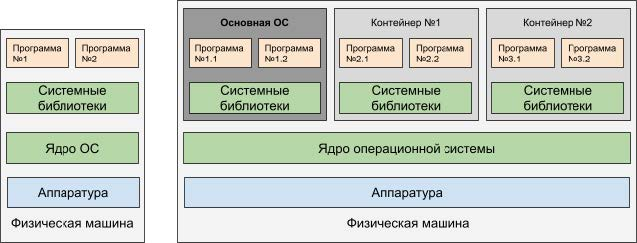
\includegraphics[width=1\textwidth]{imgs/1.1.jpg}}
    \label{framework} %framework,fig1
\end{figure}


\subsubsection*{\textbf{cgroups}}
\addcontentsline{toc}{subsubsection}{cgroups}

Управление ресурсами обеспечивается благодаря механизму cgroups (сокращение от control groups).
Обратите внимание, что все буквы в названии строго строчные. По сути, этот механизм позволяет
задать ограничения для иерархической группы процессов на использование того или иного ресурса в
системе. На дочерние процессы будут распространяться те же ограничения, что были заданы для
родительского процесса. В нынешней реализации cgroups к таким ресурсам относятся центральный
процессор, память, полоса пропускания устройств ввода-вывода и т. д. Благодаря этому можно
контролировать количество ресурсов, используемое контейнером, и, в частности, избегать ситуаций,
когда один из контейнеров единолично использует какой-то ресурс в ущерб другим контейнерам,
запущенным на данной машине. \href{https://lwn.net/Articles/256389/}{Механизм cgroups принят в ядро Linux} версии 2.6.24 в 2007 году.\\


\begin{centering}
    \subsubsection*{namespaces}
    \addcontentsline{toc}{subsubsection}{namespaces}
\end{centering}

Технология namespaces («пространства имён»), создаёт абстракцию единоличного владения неким
ресурсом для группы процессов. Несколько совершенно разных процессов могут считать, что их PID
(Process ID) равен 1. В рамках обычной системы это невозможно, так как каждый процесс с точки
зрения ОС имеет свой уникальный PID — именно в этом его смысл. Благодаря namespaces ядро ОС
может создать желаемую «видимость» для процессов или их групп.

В настоящее время доступно несколько пространств имён. Например:
\begin{enumerate}
    \item \textbf{Файловая система (mount)}: группа процессов работает со своим собственным деревом
    файловой системы. В чём-то похоже на системный вызов chroot, но в более безопасном виде:
    процессам гораздо проще «выбраться» из chroot.
    \item \textbf{UTS} (расшифровывается как Unix Time Sharing, но не имеет никакого отношения к времени):
    для каждой группы процессов позволяет задать уникальное имя хоста и домена.
    \item \textbf{Сети}: позволяет каждой группе процессов иметь свои собственные сетевые интерфейсы,
    адреса, правила обработки пакетов и т. д.\\
\end{enumerate}


% \begin{centering}
    \subsubsection*{\textbf{LXC и LXD}}
    \addcontentsline{toc}{subsubsection}{LXC и LXD}
% \end{centering}

Реализация механизмов cgroups и namespaces дала возможность создать первую технологию
контейнеров на базе оригинального ядра Linux LXC (аббревиатура от Linux containers). Безусловно,
контейнеры OpenVZ/Virtuozzo появились задолго до LXC и тоже использовали ядро.


LXC версии 0.1.0 выпущен летом 2008 года, а выпуск версии 1.0 состоялся лишь в феврале 2014
года. Отметим, что LXD — это не ещё одна реализация LXC, а всего лишь набор инструментов для
удобного управления контейнерами LXC, разрабатываемый компанией Canonical.\\


\subsubsection*{\textbf{Docker}}
\addcontentsline{toc}{subsubsection}{Docker}

В отличие от LXC, Docker — это не только и не столько демон, который позволяет создавать и
запускать контейнеры. Это полноценная экосистема, предназначенная для создания,
распространения и развёртывания приложений, упакованных в контейнеры.\\


\subsection*{Контейнеры vs VM}
\addcontentsline{toc}{subsubsection}{Контейнеры vs VM}

\begin{figure}[h]%current location
    \centering
    \scalebox{1}{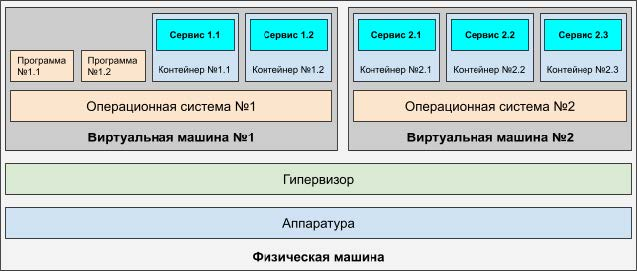
\includegraphics[width=1\textwidth]{imgs/1.2.jpg}}
    \caption*{\textit{Архитектура реального решения с использованием контейнеров внутри виртуальной машины}}
    \label{framework} %framework,fig1
\end{figure}


Выше мы рассмотрели некоторые важные особенности контейнеров, которые делают их
привлекательным средством развёртывания отдельных приложений и сервисов. В смысле
потребления системных ресурсов запуск приложения в контейнере мало чем отличается от запуска
того же самого приложения непосредственно в окружении хозяйской ОС, то есть без контейнеров.
Благодаря этому достигается высочайшая плотность использования виртуализованных приложений
на одной системе и минимизируется время развёртывания сервисов, вплоть до нескольких секунд.
При этом остаётся возможность для каждого приложения внутри контейнера создать своё
собственное окружение с файлами конфигурации, переносить контейнер вместе со всем окружением
с одной системы на другую или даже распространять таким образом преднастроенные контейнеры
как готовый к использованию продукт.

Но, как это часто бывает, обратная сторона преимуществ оказывается недостатками. Как отмечалось
ранее, невозможно запустить контейнеры, предназначенные для разных хозяйских ОС, в одной
системе. Запуск разных ОС на нескольких виртуальных машинах мы пока оставим за скобками. Опять
же, по природе своей контейнеры изолированы друг от друга значительно слабее, чем виртуальные
машины: все контейнеры используют одно и то же ядро ОС.

Тем не менее, контейнеры определённо заслуживают своё место под солнцем, и в ряде случаев
именно они — оптимальный выбор.\newpage


\section*{Изоляция гипервизора и гостевых систем}
\addcontentsline{toc}{section}{Изоляция гипервизора и гостевых систем}


Обсудив «легковесную» виртуализацию на уровне операционной системы, можно начать изучение
полноценных (по сравнению с контейнерами, «тяжеловесных») виртуальных машин.

Как реальная вычислительная машина требует первоначальной сборки, настройки, запуска и
дальнейшего обслуживания, так и виртуальная машина, будучи абстракцией машины реальной, не
может обходиться без внешнего управления. Более того, в отличие от реальной машины, аппаратура
которой используется в один момент времени одним набором ПО, каким бы он сложным ни был,
виртуальные машины делят одну и ту же аппаратуру с другим ПО. В результате получается
конструкция, как на иллюстрации ниже:

\begin{figure}[h]%current location
    \centering
    \scalebox{0.7}{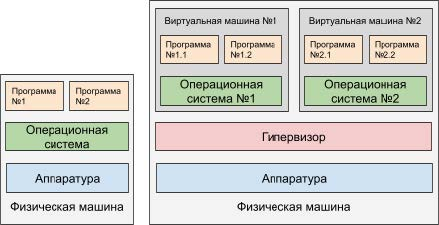
\includegraphics[width=1\textwidth]{imgs/2.1.jpg}}
    \label{framework} %framework,fig1
\end{figure}

На аппаратуре в первую очередь запускается самое важное и самое привилегированное ПО, которое
имеет полный (насколько это возможно) доступ к аппаратуре. Традиционно в роли такого ПО
выступало ядро операционной системы. Чтобы ядро ОС могло напрямую управлять доступной
аппаратурой, оно запускается и выполняется в специальном режиме. Его называют режимом ядра (от
англ. kernel mode) или режимом супервизора (от англ. supervisor — «наблюдатель, смотритель,
руководитель»).

Выполнив необходимую инициализацию аппаратуры, ядро запускает приложения пользователя в
непривилегированном или так называемом пользовательском режиме (от англ. user mode). Таким
образом обеспечивается защита системы от злонамеренных или неверно функционирующих
программ. Стоит обратить внимание на то, как выполнено разграничение между ядром ОС и
процессами в пользовательском пространстве (от англ. user space). Такое разграничение стало
возможным благодаря использованию специально предусмотренного режима работы центрального
процессора. Он появился как ответ на желание изолировать пользовательское ПО от низкоуровневого
системного.


\begin{figure}[h]%current location
    \centering
    \scalebox{1}{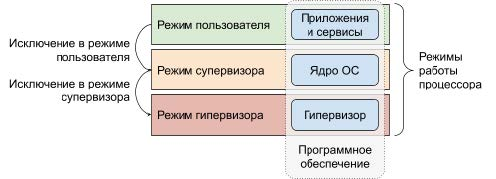
\includegraphics[width=1\textwidth]{imgs/2.2.jpg}}
    \caption*{\textit{Выполнение ПО в разных режимах работы процессора}}
    \label{framework} %framework,fig1
\end{figure}

В случае использования виртуальных машин ситуация существенно усложняется. Во-первых, потому
что появляется ещё один уровень абстракции между реальной аппаратурой и полноценной
операционной системой внутри виртуальной машины. Этот компонент принято называть монитором
виртуальных машин (англ. VMM — Virtual Machine Monitor) или гипервизором (англ. hypervisor). Это, по сути, супервизор над
супервизором — тут имеется в виду ядро ОС гостевой системы.

Если разделение между гипервизором и операционной системой можно было бы реализовать,
используя всё те же два режима работы процессора (режим ядра и пользовательский режим), то как
тогда изолировать ядро ОС внутри виртуальной машины от гипервизора? А сделать это необходимо: в
противном случае виртуальная машина будет способна влиять на работу других виртуальных машин
и на всю систему в целом. Вторая сложность возникает в случае запуска нескольких виртуальных
машин на одной аппаратуре. Тогда нужно изолировать гостевые системы друг от друга.

Осталось разобраться, каким образом возможно реализовать изоляцию между гипервизором и
гостевыми системами. Тут стоит вернуться к базовым принципам функционирования центрального
процессора (ЦП). По большому счёту, всё, что делает ЦП, — это загружает из памяти команды и
операнды (данные, над которыми будут выполняться какие-то операции), выполняет необходимые
операции (вычисления) и при необходимости сохраняет результат операции в память. Это значит, что
для разделения режимов исполнения ПО (режимов пользователя, супервизора и гипервизора) в
первом приближении достаточно лишь разделить области памяти, которые используются в разных
режимах.

Действительно, если программа, работающая в пользовательском режиме, не сможет получить
доступ к коду ядра ОС или же гипервизора, то проблему можно считать решённой. Более того, при
использовании концепции виртуальной памяти со страничной организацией доступ к различным
частям памяти может быть очень гибко ограничен. Страничная организация означает, что для каждой
страницы (блока памяти фиксированного размера, как правило, 4, 8 или 16 Кб) возможно задавать
права доступа с точностью до единичного процесса в системе.

Такое приближение не учитывает одной важной детали: в некоторых случаях операции, выполняемые
процессором, требуют взаимодействия с аппаратурой. Самый простой пример — возникновение 
исключительной ситуации при делении на ноль. В случае работы единственной ОС на железе
происходит вызов процедуры обработки исключительной ситуации. В результате её выполнения ОС
может принять решение преждевременно завершить пользовательскую программу.

Пикантность ситуации заключается в том, что такой обработчик исключительной ситуации
регистрируется только один для всей системы. При этом обработчик является частью хозяйского ПО:
основной ОС или гипервизора. И мы сталкиваемся с парадоксальной ситуацией: гостевая ОС при
всём желании не может установить в системе свой обработчик исключительной ситуации из-за
использования ЦП в режиме ограниченных привилегий, однако обработка исключительной ситуации
будет происходить в соответствующем обработчике, являющимся частью хозяйского ПО.\\


\subsection*{Привилегированные и служебные команды процессора}
\addcontentsline{toc}{subsection}{Привилегированные и служебные команды процессора}

Мы можем сделать вывод, что гостевой системой хоть и редко, но могут производиться операции,
требующие расширенных полномочий, если мы хотим, чтобы она была настолько же полноценной,
как и её вариант, запущенный непосредственно на аппаратуре. В противном случае мы придём к так
называемой паравиртуализации. Как правило, речь идёт о выполнении команд процессора,
способных влиять на важные состояния аппаратуры: менять режимы работы процессора, включать и
отключать обработку прерываний, получать доступ ко внешним аппаратным блокам. Такие команды
процессора удобно называть служебными. Название «служебные команды» было предложено
Попеком и Голдбергом в их работе Formal Requirements for Virtualizable Third Generation Architectures.

Строго говоря, любая выполняемая процессором команда, независимо от режима работы и
имеющихся в данный момент привилегий, изменяет состояние процессора. Даже при выполнении
команды NOP (от англ. No OPeration — «отсутствие действия») изменяется как минимум счётчик
команд, который после выполнения текущей команды указывает на следующую. В процессорах с
архитектурой x86 это регистр EIP.

Как показали Попек и Голдберг, если служебные команды являются подмножеством
привилегированных команд, то можно весьма эффективно обеспечить виртуализацию гостевых
систем. Достаточно выполнять все команды гостевого ПО в исходном виде непосредственно на
реальном процессоре, переключаясь в режим эмуляции только для выполнения привилегированных
команд. В противном случае гипервизор должен перед выполнением следующего блока кода
убедиться, что в этом блоке не содержится служебных команд, которые нельзя выполнять
непосредственно, а нужно их эмулировать. Так было с процессорами Intel семейства x86 до
появления расширения VT-x. Очевидно, такой режим работы требует большей вовлечённости
гипервизора, а потому эффективность виртуализации существенно снижается.\\

\subsection*{Доступ к памяти и аппаратуре}
\addcontentsline{toc}{subsection}{Доступ к памяти и аппаратуре}

Современные ОС общего назначения используют абстракцию виртуальной памяти с разделением на
страницы. Это даёт возможность устанавливать права доступа к произвольным областям физической
памяти с гранулярностью, соответствующей размеру страницы MMU (сокр. от англ. Memory
Management Unit). Таким образом можно реализовать абстракцию адресных пространств, уникальных
для каждого процесса в системе.

Современные процессоры с архитектурой x86 и ARM имеют базовый размер страницы MMU, равный
4 Кб, что не мешает объединять их в группы большего размера. Например, компания Apple в свежих
версиях iOS оперирует размером страницы памяти в ОС, равным 16 Кб, хотя на аппаратном уровне
используются всё ещё страницы размером 4 Кб.

Для обеспечения работы виртуальной памяти необходимо настраивать правила трансляции
виртуальных адресов в физические, не забывая устанавливать соответствующие права доступа для
каждой страницы, для которой устанавливается правило трансляции. Поскольку фактически
трансляция адресов происходит непосредственно в аппаратуре (этим как раз и занимается MMU), то
лишь хозяйская ОС или гипервизор должны иметь возможность устанавливать и менять правила
трансляции. А гостевые системы внутри виртуальных машин, имея желание самим задавать
трансляции, должны получать желаемое в результате эмуляции их запроса гипервизором.

В данном случае важно, что установка и изменение таблицы трансляции случается в процессе
работы современной ОС общего назначения относительно часто. А потому эффективность работы
гипервизора, выполняющего эмуляцию данных запросов гостевых систем, в значительном объёме
влияет на эффективность виртуализации в целом.\newpage



\section*{Бинарная трансляция и паравиртуализация}
\addcontentsline{toc}{section}{Бинарная трансляция и паравиртуализация}

\subsection*{Бинарная трансляция}
\addcontentsline{toc}{subsection}{Бинарная трансляция}

Как показано выше, гипервизору так или иначе приходится обслуживать некоторые запросы гостевых
систем, которые те не могут выполнить самостоятельно из-за своих ограниченных привилегий.
Наиболее очевидный способ выполнения запросов гостя — эмуляция. В самом простом виде
эмуляцию можно реализовать в виде трансляции каждой команды гостевой системы.\\

Происходит это следующим образом:

\begin{enumerate}
    \item Гипервизор загружает бинарный образ ПО, которое должна выполнить гостевая система.
    \item Начиная с «точки входа», гипервизор декодирует команды гостя: обнаруживает границы
    первой команды, определяет её длину, ищет её описание в «базе данных» известных
    интерпретатору команд.
    \item Выполняет действия, которые предполагает данная команда.
    \item Сохраняет существенные для дальнейшей работы интерпретатора изменения внутреннего
    состояния интерпретатора и данные, над которыми были произведены действия.
    \item Загружает следующую команду в соответствии с ходом выполнения команд. Если предыдущая
    команда предусматривала изменение хода выполнения программы (условный, с
    выполненным условием или безусловный переход), то следующая команда будет загружена с
    адреса, куда был осуществлён переход. В противном случае будет загружена следующая
    команда из бинарного образа программы.
    \item Декодируется и выполняется новая команда и т. д.
\end{enumerate}

Даже из этого перечня операций становится понятно, что на каждую команду эмулируемого
процессора хозяйская система выполняет большое количество операций. Соответственно, скорость
выполнения программы гостевой системы значительно снижается по сравнению со скоростью её
выполнения на реальной системе. И речь тут идёт, к сожалению, не о разах, а о порядках. Ни о какой
эффективности при таком подходе говорить не приходится.

Тем не менее полная эмуляция может находить себе применение. Самое очевидное из них —
эмуляция нового оборудования, в особенности процессоров с новым набором команд (ISA —
Instruction Set Architecture). Простейший эмулятор для новой процессорной архитектуры можно
реализовать очень быстро и начать разработку системного ПО для новых процессоров задолго до
появления реальной аппаратуры. В данном случае скорость работы отступает на второй план, важнее
сама возможность запускать на выполнение код.

Однако вернёмся к вопросам эффективной виртуализации, для которой важно исполнение гостевого
кода с минимальными накладными расходами. Как можно ускорить трансляцию кода гостевой
системы? Один из очевидных вариантов — сохранение и повторное использование результатов
интерпретации ПО гостевой системы. Действительно, гипервизор исполняется на хозяйской системе в
виде набора команд хозяйского процессора, и, соответственно, команды ПО гостевой системы в
результате трансляции преобразуются в набор команд для хозяйского процессора. А значит, можно
поставить в соответствие каждой эмулируемой команде набор команд хозяйской системы и при
повторном исполнении команды гостевого процессора выполнять заранее известный набор команд
хозяйской системы.

Пока ни о каком повышении эффективности речи не идёт, так как для каждой гостевой команды всё
ещё происходит выполнение всё того же количества хозяйских команд. Но можно произвести
трансляцию и оптимизацию соответствующих команд для хозяйской системы не для одной
инструкции, а сразу для «базового блока» — набора команд, всегда исполняемых линейно, то есть
без изменения хода выполнения внутри. В данном случае возможно сэкономить значительное
количество команд хозяйской системы за счёт исключения повторяющихся операций (загрузки и
декодирования команд, сохранения промежуточных результатов), а также за счёт оптимизаций,
специфичных для хозяйской системы: переупорядочивания команд, более эффективного
использования регистров процессора, кешей и т. д.

Подобным образом работают современные высокопроизводительные эмуляторы, такие как QEMU. В
зависимости от исполняемого ПО, 
\href{https://pyra-handheld.com/boards/threads/qemu-emulation-performance-for-different-guest-architectures.80772/}{эмуляция в QEMU} 
может быть в несколько раз (и даже в десятки
раз) медленнее, чем на реальной системе. Это всё ещё очень неэффективно, но, во-первых, этим уже
можно пользоваться, имея достаточно производительную хозяйскую систему. А во-вторых, как
отмечалось выше, полная бинарная трансляция позволяет выполнять ПО, скомпилированное для
платформ и даже архитектур (ISA), полностью отличных от хозяйской. Например, ПО для популярной
платы Raspberry Pi, построенной на базе процессора с системой команд ARM, можно запустить в
QEMU на машине с процессором Intel. 

Если же ограничиться выполнением ПО, скомпилированного для процессора, совпадающего по
набору команд с процессором хозяйской системы, можно сделать ещё одну оптимизацию: выполнять
бинарную трансляцию только частей кода, содержащих команды, которые требуют особенного
внимания (см. выше критерий Попека-Голдберга). Поскольку таких команд (в терминологии
Попека-Голдберга — «служебных» и «привилегированных») относительно немного, то большую часть
кода гостя можно исполнять, как если бы это было обыкновенное приложение, запущенное в гостевой
системе, то есть без какой-либо трансляции. Именно так работают Oracle VirtualBox и VmWare
Workstation в режиме работы без аппаратного ускорения виртуализации. И при этом
производительность гостевой системы может приближаться к производительности реальной системы.

Тем не менее не стоит забывать, что в зависимости от запускаемого в гостевой системе ПО,
вовлечённость гипервизора может значительно варьироваться. То есть в некоторых случаях
производительность гостевой системы может существенно снижаться.\\

\subsection*{Паравиртуалиация}
\addcontentsline{toc}{subsection}{Паравиртуалиация}

До сих пор мы рассматривали ситуации с запуском немодифицированного ПО в окружении гостевой
системы. Это удобно, потому что даёт возможность запускать всё что угодно: от простых примеров на
ассемблере, которые выполняют простейшие действия вроде сложения двух констант в регистрах
процессора, до полноценных ОС на вкус пользователя.

Тем не менее, если наша цель — максимально эффективно выполнять определённые задачи в
виртуализованном окружении, стоит попробовать оптимизировать то самое ПО, которое запускается в
гостевой системе. Такой подход называется паравиртуализацией. Суть её сводится к тому, что ПО
гостевой системы изменяется таким образом, чтобы использовать некоторые особенности
гипервизора.

Например, типичный способ коммуникации гостевой системы с внешним миром и даже хозяйской
системой реализуется при помощи сетевого подключения. Для этого гипервизор реализует модель
некоторого реального контроллера сети Ethernet, например RTL8139, с большим количеством
деталей: регистров управления, внутренних состояний, буферов для обмена данными при помощи
DMA (Direct Memory Access), прерываний и т. д. А гостевая система при помощи имеющегося
стандартного драйвера использует предоставленную модель устройства.

Такое усложнение с обеих сторон (со стороны гипервизора и гостевой системы) определённо не идёт
на пользу эффективности использования вычислительных ресурсов аппаратуры. Вместо этого можно
использовать специально созданное для виртуальной машины устройство, которое будет иметь
упрощённую структуру, поскольку фактически никакого сетевого контроллера и не существует, а
происходит обмен блоками данных в памяти реальной системы между гипервизором и гостем.
Хороший тому пример — \href{https://developer.ibm.com/articles/l-virtio/}{Virtio-устройства}. 
Virtio представляет собой абстракцию устройства,
предназначенного для использования гипервизорами. На сегодняшний день Virtio используется по
умолчанию гипервизорами KVM и Xen.


\begin{figure}[h]%current location
    \centering
    \scalebox{0.7}{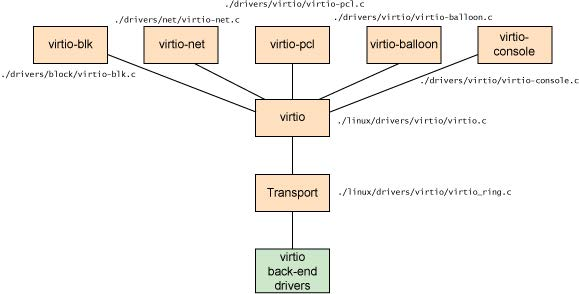
\includegraphics[width=1\textwidth]{imgs/3.1.jpg}}
    \caption*{\textit{Высокоуровневая архитектура фреймворка Virtio}}
    \label{framework} %framework,fig1
\end{figure}

Паравиртуализованные устройства — самый простой и весьма продуктивный способ повышения
эффективности виртуализации. Ввод-вывод данных составляет значительную часть реальной работы
многих приложений, а добавить в имеющуюся ОС драйвер нового устройства (например, Virtio-диска
или сетевого контроллера) не составляет труда и не требует модификации ядра ОС. То есть всё ещё
возможно использовать ОС без специальной адаптации.

Тем не менее, паравиртуализации подвергают и другие части системы: таймеры, подсистему
обработки прерываний, систему управления виртуальной памятью (MMU) и даже планировщик задач.

\begin{figure}[h]%current location
    \centering
    \scalebox{0.7}{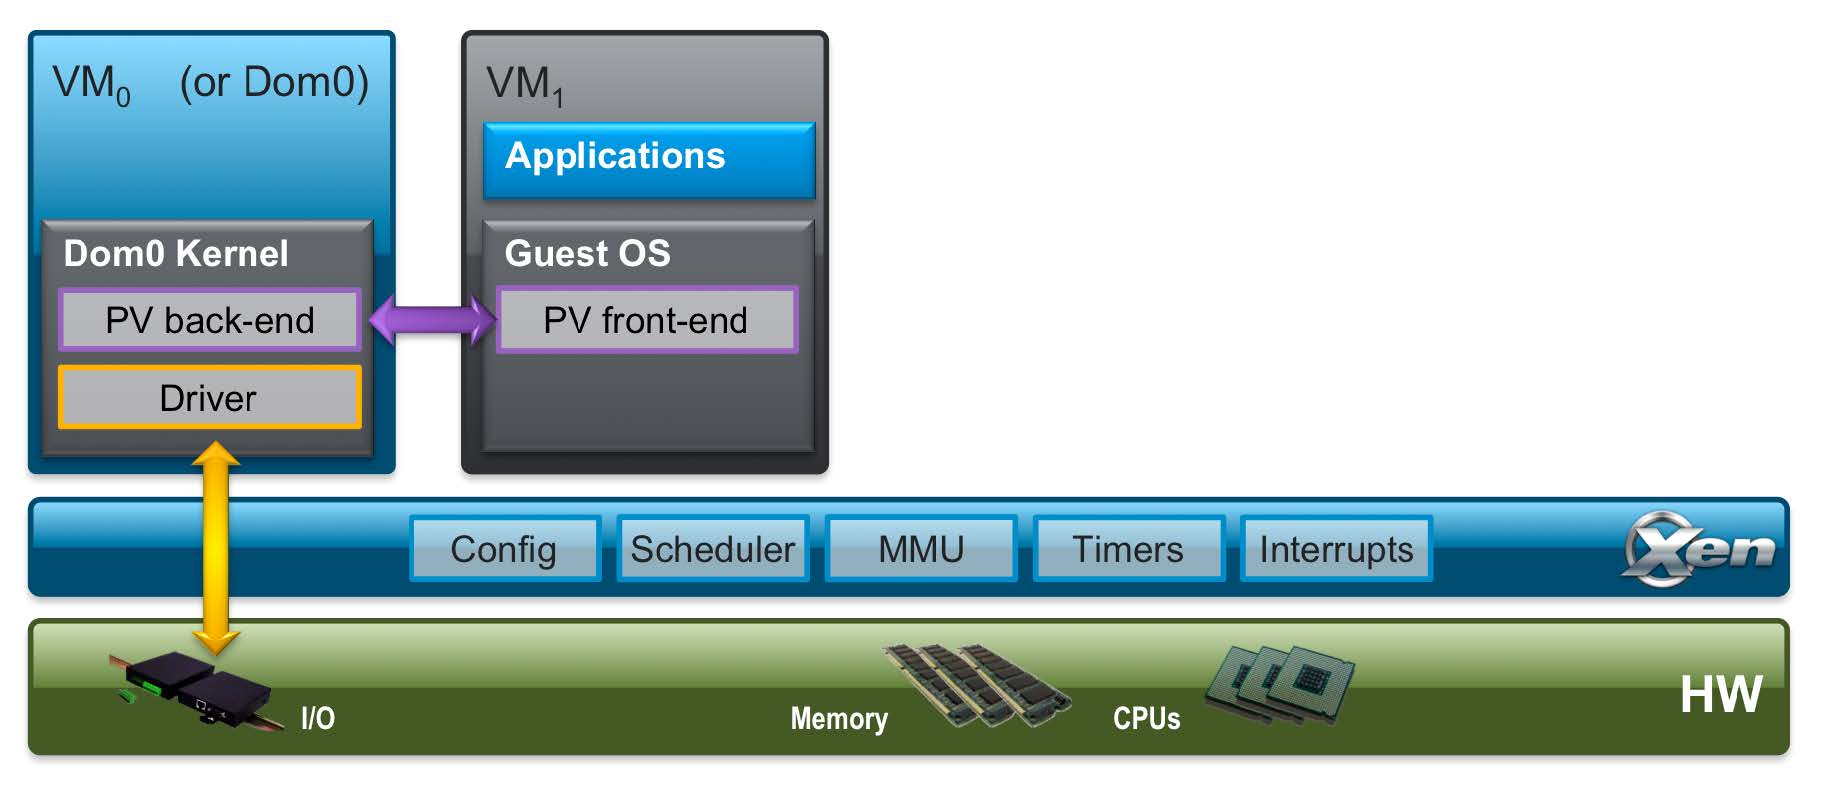
\includegraphics[width=1\textwidth]{imgs/3.2.jpg}}
    \caption*{\textit{Паравиртуализация оборудования в гипервизоре Xen}}
    \label{framework} %framework,fig1
\end{figure}

Например, существуют ядра ОС Linux и нескольких разновидностей BSD, которые поддерживают
полную паравиртуализацию в гипервизоре XEN.

Но стоит отметить, что «полная» паравиртуализация в настоящее время уступила пальму первенства
комбинированной виртуализации — использованию аппаратной поддержки виртуализации вместе с
паравиртуализованными устройствами ввода-вывода. Таким образом, берётся «лучшее из обоих
миров»: возможность запускать немодифицированное ядро ОС с высокой эффективностью за счёт
аппаратной поддержки виртуализации (об этом чуть ниже) и высокоэффективный ввод-вывод. \newpage


\section*{Аппаратная поддержка виртуализации в современных процессорах}
\addcontentsline{toc}{section}{Аппаратная поддержка виртуализации в современных процессорах}

Как уже упоминалось, серверная виртуализация появилась несколько десятилетий назад и долгое
время оставалась прерогативой огромных и очень дорогих машин — mainframe. Но с бурным ростом
парка x86-совместимых компьютеров и их захватом значительной доли рынка серверов средства
серверной виртуализации получили своё развитие на платформе, первоначально предназначенной
для персонального использования. Речь идёт о дальних потомках компьютеров серии IBM PC,
которые были построены на процессорах Intel 8088.

\href{http://www.usenix.org/events/sec2000/robin.html}{Исследования показали},
что процессоры Intel семейства x86 имеют фундаментальные проблемы с
реализацией эффективной виртуализации на уровне аппаратуры: 18 «служебных» команд
процессора не были «привилегированными». Это потребовало выполнять сканирование кода,
предназначенного для выполнения гостевой системой выборочной бинарной трансляции, что снизило
эффективность такой виртуализации. Закономерным было и то, что x86-совместимые процессоры
компании AMD страдали от того же самого недостатка.\\


\subsection*{Intel VT}
\addcontentsline{toc}{subsection}{Intel VT}

Когда популярность виртуализации на платформе x86 стала очевидной, компания Intel разработала
целый набор усовершенствований для своих процессоров под общим названием Intel Virtualization
Technology, или сокращённо Intel VT. Первые процессоры с поддержкой первой версии Intel VT
расширений появились в 2005 году, это были Pentium 4 (модели 662 и 672). Во время разработки
технология носила название Vanderpool.

\subsubsection*{\textbf{VT-x (Intel Virtualization Technology)}}
\addcontentsline{toc}{subsubsection}{VT-x (Intel Virtualization Technology)}

Intel 32-bit architecture, реализованная в семействе x86-процессоров, сокращённо называется IA-32.
Важнейшая особенность архитектуры IA-32 — обратная совместимость, то есть возможность на
более новых процессорах запускать ПО, разработанное и скомпилированное для более старых
процессоров того же семейства. Компания Intel была заинтересована в сохранении этой особенности.

Вместо создания нового набора команд, лишённого такого недостатка, как непривилегированные
служебные команды, Intel добавила ещё один режим работы процессора — VMX. Можно его
представить как минус первое кольцо защиты, то есть находящееся внутри нулевого кольца защиты, в
котором традиционно выполняется ядро ОС. В этом новом режиме работы, также ещё называемом
«режим гипервизора», происходит настройка гостевого окружения, и в дальнейшем, после запуска
гостевой системы, обрабатываются ситуации, которые намеренно недоступны для обработки гостевой
системой.

\begin{figure}[h]%current location
    \centering
    \scalebox{0.7}{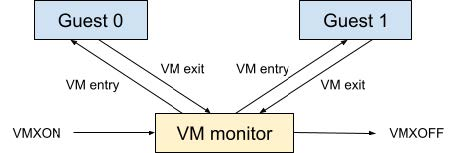
\includegraphics[width=1\textwidth]{imgs/4.1.jpg}}
    \label{framework} %framework,fig1
\end{figure}

Красота такого решения в том, что гостевая система при всём желании не может узнать, что она
запущена в каком-то особенном режиме и помимо неё в системе могут существовать другие гости или
гипервизор. Тем самым достигается возможность запускать в гостевом окружении любое ПО.

Причём гипервизор может с высокой точностью настроить гостевое окружение благодаря структуре
VMCS (сокр. от англ. Virtual Machine Control Structure). В основном настройка сводится к указанию
ситуаций, при которых происходит так называемый VM exit — выход из режима гостя в гипервизор для
обработки конкретного события, такого как внешнее прерывание, исключительная ситуация и т. д.

Важно отметить, что упомянутый VM exit и следующее за ним VM entry (возвращение в режим гостя)
— это очень дорогостоящие операции с точки зрения общей производительности системы, так как
происходит, в сущности, полноценное переключение контекста. Приходится сохранять одно состояние
в память, восстанавливать другое, а затем проделывать всё это в обратном порядке. Поэтому чем
реже случаются VM exit и VM entry, тем эффективнее работает система. А для этого нужно дать
возможность гостевой системе обрабатывать как можно больше особенных ситуаций.

Это, в свою очередь, становится возможным с дальнейшим совершенствованием аппаратной
поддержки виртуализации. В 2008 году компания Intel выпустила процессоры с микроархитектурой
Nehalem, некоторые из которых имели поддержку EPT (Extended Page Tables) — таблицу трансляции
«физических» адресов гостевой системы в реальные физические адреса системы. EPT существенно
повышает производительность работы подсистемы виртуальной памяти гостевых систем. В
\href{http://www.vmware.com/pdf/Perf_ESX_Intel-EPT-eval.pdf}{Performance Evaluation of Intel EPT Hardware Assist}
отмечается увеличение производительности тестов, активно использующих MMU, до 48%.

В 2012 году Intel представила решение для виртуализации прерываний — APIC virtualization. APIC
расшифровывается как Advanced Programmable Interrupt Controller.

В 2013 году с анонсом микроархитектуры Haswell компания Intel представила возможность
использования «затенения» (англ. shadowing) структуры VMCS, что открыло возможности для
реализации вложенной виртуализации.\\

\subsubsection*{\textbf{VT-d (Virtualization technology for directed I/O)}}
\addcontentsline{toc}{subsubsection}{VT-d (Virtualization technology for directed I/O)}

Как мы отмечали ранее, ввод-вывод данных — это неотъемлемая часть работы современной
компьютерной системы, а потому накладные расходы на ввод-вывод заметно сказываются на общей
производительности системы. Действительно, как бы быстро ни происходили вычисления, если
приходится ожидать загрузки данных для обработки, то общая скорость выполнения задачи падает.

Для высокоскоростного ввода-вывода традиционно используется DMA (Direct Memory Access) —
предоставление периферийному устройству возможности записи или чтения данных непосредственно
в память или из памяти. Для работы при помощи DMA процессор выделяет буфера в памяти и
передаёт указатели на них периферийному устройству. Оно по мере необходимости записывает или
считывает данные из этих буферов и сигнализирует центральному процессору о выполнении той или
иной операции при помощи прерываний.

Сложности возникают при конфигурации DMA из гостевого окружения виртуальной машины. С одной
стороны, гостевая система по определению не должна иметь возможности работать с физической
памятью напрямую. Гостевая система использует виртуализированные ресурсы и, в частности,
память. А с другой стороны, реальное периферийное устройство (такое как контроллер сети Ethernet)
работает с памятью напрямую, используя реальные физические адреса. То же касается и
прерываний: с одной стороны, гостевая система не должна напрямую заниматься обработкой
прерываний, а с другой стороны, периферийное устройство использует реально существующие в
системе линии прерываний.

Без аппаратной поддержки эффективного ввода-вывода при виртуализации гипервизор выполняет
полную эмуляцию устройства. При этом настройкой DMA-транзакций занимается гипервизор, он же
первоначально обрабатывает прерывания от устройства, по мере необходимости вызывая
обработчики прерываний гостевой системы. Тут важно вспомнить, что каждое переключение из
режима гостя в режим гипервизора и обратно дорого обходится в смысле производительности всей
системы.

\begin{figure}[h]%current location
    \centering
    \scalebox{0.7}{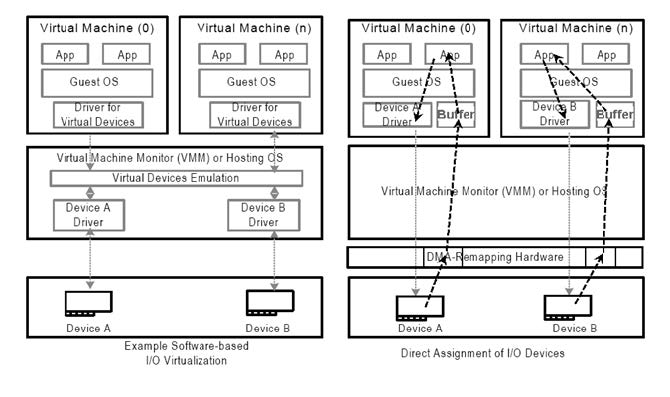
\includegraphics[width=1\textwidth]{imgs/4.2.jpg}}
    \caption*{\href{https://software.intel.com/en-us/articles/intel-virtualization-technology-for-directed-io-vt-d-enhancing-intel-platforms-for-efficient-virtualization-of-io-devices}{\textit{Software Emulation based I/O vs. Hardware based Direct Assignment I/O}}}
    \label{framework} %framework,fig1
\end{figure}

Решение этой проблемы состоит в таком усовершенствовании аппаратуры, когда, будучи
сконфигурированной гипервизором, она «на лету» автоматически производит преобразование
адресов, используемых для доступа к памяти. То есть гостевая система, как и раньше, знать ничего не
знает о физической памяти, однако внешнее периферийное устройство получает реальные
физические адреса. Что-то похожее касается и прерываний: гипервизор имеет возможность для
каждого реального прерывания указать гостевую систему, обработчик из которой должен быть вызван.
Таким образом гипервизор почти полностью исключается непосредственно из процесса обмена
данными между гостевой системой и периферийным устройством.

В данном случае речь идёт об усовершенствовании не только процессора, но и внешних по
отношению к нему компонентов, таких, например, как контроллер памяти. А потому для
использования технологии Intel VT-d необходимо иметь систему, состоящую из соответствующих
процессора и чипсета, — оба должны поддерживать VT-d. Стоит иметь в виду, что в реальной жизни
чипсеты для настольных и мобильных систем (ноутбуков) могут запросто не иметь поддержки VT-d.
При этом поддержка VT-d процессором не играет никакой роли, то есть можно считать, что такая
система не поддерживает эффективный ввод-вывод для виртуализации.

В случае возникновения ошибок, вызванных неправильной настройкой или попыткой доступа к
запрещённым ресурсам, гипервизор всё равно вступает в игру для урегулирования ситуации. Но,
хочется надеяться, такое случается весьма редко, а потому не влияет на общую эффективность
системы, использующей VT-d.\\

\subsection*{\textbf{Прочие улучшения}}
\addcontentsline{toc}{subsection}{Прочие улучшения}

Со временем появляются всё более сложные и интересные решения для повышения эффективности
виртуализации. Ниже перечислено несколько относительно свежих разработок компании Intel.

\begin{enumerate}
    \item \textbf{IntelR Graphics Virtualization Technology (Intel GVT)} — серия улучшений для виртуализации
    графических контроллеров.
    \begin{enumerate}
        \item[a.] \textbf{Intel GVT-d} позволяет передать управление графическим процессором (англ. graphics
        processing unit, GPU) одному конкретному гостю.
        \item[b.] \textbf{Intel GVT-s} позволяет нескольким гостям совместно использовать один и тот же
        графический контроллер при помощи специфического драйвера в гостевой системе.
        \item[c.] \textbf{Intel GVT-g} — некая смесь первых двух вариантов. В один момент времени только
        один гость имеет полный контроль над графическим контроллером, как если бы
        реальный графический контроллер был частью данной виртуальной машины. А
        гипервизор производит переключение GPU между гостями, давая каждому гостю
        некоторый отрезок времени для работы напрямую с GPU.
    \end{enumerate}
    \item \textbf{Intel Virtualization Technology for Connectivity} — усовершенствования для эффективной
    виртуализации высокопроизводительных сетевых контроллеров. Позволяют нескольким
    гостям одновременно работать с одним сетевым контроллером.
\end{enumerate}

\subsection*{\textbf{AMD-V}}
\addcontentsline{toc}{subsection}{AMD-V}

Разумеется, всё те же ограничения, связанные с виртуализацией, относились и к процессорам
производства компании AMD, поскольку они реализовывали тот же набор команд, что и процессоры
Intel семейства x86. Неудивительно, что AMD практически одновременно с Intel разработала набор
расширений для повышения эффективности виртуализации под кодовым именем Pacifica.
Расширения тем не менее были выпущены с процессорами Athlon 64 в мае 2006 года под
маркетинговым названием AMD Secure Virtual Machine, а позже переименованы в AMD Virtualization
или просто AMD-V. Хотя AMD использует несколько отличную от Intel терминологию, смысл
реализованных расширений во многом совпадает. Введён новый режим для работы гипервизора —
host mode (гостевые системы запускаются в guest mode), добавлены новые команды для запуска
гостевой ОС и управления структурой данных, содержащей информацию о состоянии гостевой
системы и т. д.

Так же, как и Intel, AMD позже разработала расширения для виртуализации подсистемы виртуальной
памяти AMD Rapid Virtualization Indexing (RVI), подсистемы прерываний AMD AVIC Advanced Virtual
Interrupt Controller (AVIC) и подсистемы ввода-вывода AMD I/O Virtualization Technology (AMD-Vi).

\subsection*{\textbf{AMD-V}}
\addcontentsline{toc}{subsection}{AMD-V}

Хотя процессоры с системой команд ARM присутствуют на рынке много лет, до недавнего времени
они использовались в относительно маломощных портативных устройствах: сотовых телефонах,
мультимедиа-приставках и т. п. Однако в последние годы мы наблюдаем две интересные тенденции.

С одной стороны, мобильные устройства в смысле производительности вплотную приблизились к
настольным системам: существуют 64-битные многоядерные и даже многокластерные системы,
работающие на частоте 2–3 ГГц, имеющие в своём распоряжении гигабайты оперативной памяти. С
другой стороны, производители серверного оборудования не первый год пытаются вывести на рынок
полноценные ARM-серверы. В обоих случаях становится достаточно производительности для запуска
сложных задач и появляются сценарии, требующие запуска виртуальных машин. Мотивация в данном
случае всё такая же, как и ранее на «больших» компьютерах: повышение эффективности
использования аппаратных ресурсов, повышение безопасности, надёжности и т. д.

Компания ARM, так же как Intel и AMD ранее, разработала набор расширений для поддержки
эффективной виртуализации. В новой версии своей процессорной архитектуры Armv8.1 компания
реализовала Virtualization Host Extensions (VHE). В Armv8.3 добавлена поддержка вложенной
виртуализации, в Armv8.4 режим вложенной виртуализации ещё более усовершенствован.

Как мы видим, развитие технологий аппаратного ускорения виртуализации происходит постепенно и
не прекращается по сегодняшний день. Фактически разработчики микропроцессоров раз за разом
устраняют обнаруженные «узкие места», всё больше повышая эффективность виртуализации. А это
значит, что в обозримом будущем аппаратная виртуализация получит ещё большее распространение.\newpage

\section*{Практическое задание}
\addcontentsline{toc}{section}{Практическое задание}

\begin{enumerate}
    \item Назовите преимущества и недостатки контейнеров, полной виртуализации и
    паравиртуализации (полной и частичной — только устройств ввода-вывода).
    \item Установите 32-битную версию Ubuntu 16.04 в Oracle Virtualbox или в VMware Workstation Player
    в двух режимах: с использованием аппаратного ускорения виртуализации (Intel VT-x или
    AMD-V) и без. Обратите внимание на скорость загрузки системы в виртуальной машине и
    запуска различных приложений в обоих режимах.
\end{enumerate}

\section*{Используемые источники}
\addcontentsline{toc}{section}{Используемые источники}

\begin{enumerate}
    \item \href{https://pasztor.at/blog/under-the-hood-of-docker}{Janos Pasztor, Under the hood of Docker}
    \item \href{https://developer.ibm.com/articles/l-virtio}{Virtio: An I/O virtualization framework for Linux, M. Jones, IBM}
    \item \href{https://www.intel.com/content/dam/www/public/us/en/documents/manuals/64-ia-32-architectures-software-developer-vol-3c-part-3-manual.pdf}{Intel 64 and IA-32 Architectures Software Developer’s Manual Volume 3C: System Programming
    Guide, Part 3}
    \item \href{https://software.intel.com/sites/default/files/managed/fd/35/Intel%20Graphics%20Virtualization%20Update.docx}{Intel graphics virtualization update, Sunil Jain, Intel Corporation}
    \item \href{https://www.intel.com/content/dam/www/public/us/en/documents/technology-briefs/virtualization-technology-connectivity-brief.pdf}{Intel Virtualization Technology for Connectivity}
    \item \href{https://www.mimuw.edu.pl/~vincent/lecture6/sources/amd-pacifica-specification.pdf}{AMD64 Virtualization Codenamed "Pacifica" Technology, Secure Virtual Machine Architecture
    Reference Manual}
    \item \href{https://developer.arm.com/docs/ddi0487/latest/arm-architecture-reference-manual-armv8-for-armv8-a-architecture-profile}{Arm Architecture Reference Manual Armv8, for Armv8-A architecture profile}
\end{enumerate}


\end{document}
